\chapter{Orchestration Using Heat}\label{cha:orch-using-heat}
\gls{Heat} is the name of the OpenStack orchestration engine, which
can manage complete configurations of all servers, volumes, users,
networks and routers that make up a cloud application.  Instead of
managing every component separately, we can create, start, stop or
clean up our complete application in a single step.  Such a set of
collectively managed resources is called a \gls{stack}.

\gls{Heat} has its own dashboard interface, which you can find under
the \strong{Orchestration} tab of the main OpenStack dashboard.  Official
documentation for Heat and its dashboard interface can be found at the
following locations:
\begin{itemize}
\item \url{https://docs.openstack.org/heat/\osversion}
\item \url{https://docs.openstack.org/heat-dashboard/\osversion}
\end{itemize}

\section{\gls{Heat Orchestration Template}s}\label{sec:glsh-orch-templ}
A \gls{stack}'s resources and their mutual dependencies can be
specified in a text file, called a \gls{Heat Orchestration Template}
(\textsc{hot}).  The syntax of these templates conforms to the
\gls{yaml} standard, for which many text editors provide specialized
editing modes.  The following example describes a stack consisting of
a single VM:
\begin{code}{}
heat_template_version: 2018-03-02

description: Deploy a single compute instance

parameters:
  user_network:
    type: string
    label: user_network
    description: Add the required VM network
    constraints: [ custom_constraint: neutron.network ]
  user_key:
    type: string
    label: ssh_user_key
    description: Public ssh key for user authentication
    constraints: [ custom_constraint: nova.keypair ]

resources:
  my_instance:
    type: OS::Nova::Server
    properties:
      security_groups: [ default ]
      networks: [ network: { get_param: user_network } ]
      key_name: { get_param: user_key }
      image: Ubuntu_16.04_2NICs
      flavor: m1.small
\end{code}

Our example contains four main sections:
\begin{description}
\item[\texttt{heat\_template\_version}] The \textsc{hot} specification
  has evolved since its initial release.  The key
  \lstinline{heat_template_version} indicates the version of the
  syntax used in this template.  It's value can be a release date or
  (in recent version) the name of the version.
\item[\texttt{description}] A description is optional, but
  recommended.
\item[\texttt{parameters}] An optional section, \lstinline{parameters}
  allow users to configure various properties when instantiating a new
  stack, without having to edit the template itself.  A parameter
  value can be used elsewhere in the template using the function
  \lstinline{get_param}.
\item[\texttt{resources}] This section contains all the resources used
  by the Stack.  In this case, there is just a single VM instance.
\end{description}
Optional additional sections are \strong{\lstinline{parameter_groups}},
\strong{\lstinline{outputs}}, and \strong{\lstinline{conditions}}.

The
`\href{https://docs.openstack.org/heat/\osversion/template_guide}{Template
  Guide}' in the Heat documentation contains a specification of the
\textsc{hot} format, as well as information on how to describe the
various types of resources in a template.  \textsc{vsc} also provides
some example templates in the repository
\url{https://github.com/hpcugent/openstack-templates}.

\section{The Template Generator}\label{sec:template-generator}
The Heat dashboard provides a graphical interface where users can draw
templates by dragging resources onto a canvas, and connecting them.
Users can then download a template generated from this interface, or
immediately instantiate it as a stack.

\strong{Note:} Currently, there are a number of issues with the
template generator, which require manual edits to the generated
templates.  Therefore, the template generator is currently not very
useful.  We will update this section as soon as these problems are
solved.

\section{Managing stacks}\label{sec:managing-stacks}
The \strong{Stacks} button in the \strong{Orchestration} tab takes you
to the overview page where you can launch, suspend, resume and delete
stacks.
\begin{center}
  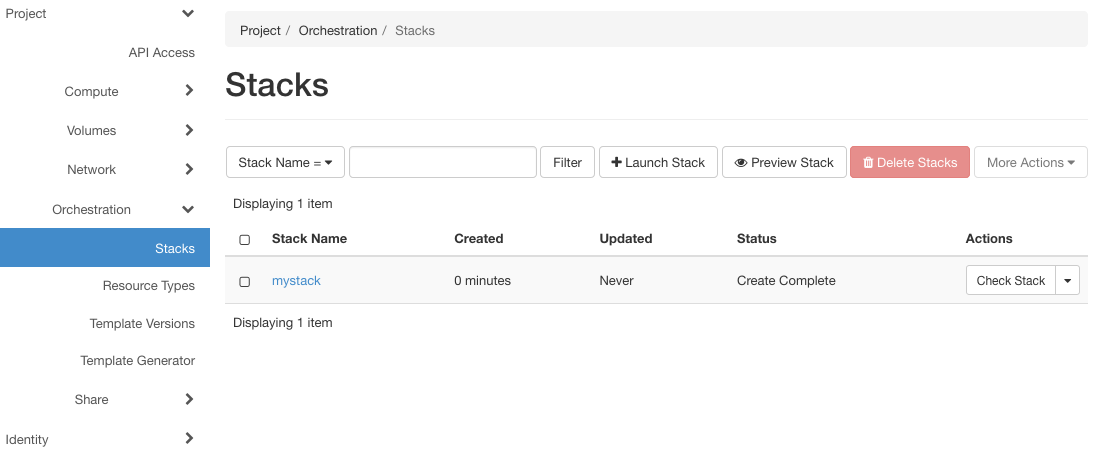
\includegraphics[width=\textwidth]{img/stacks_overview}
\end{center}
The overview page contains a list of all currently existing stacks
(either running or suspended), and buttons to perform the following
actions:

\begin{description}
\item{\strong{Launch Stack}} starts a wizard to create a stack from a
  template.  Depending on your choice of \strong{Template Source}, you
  can provide a local file on your system, directly type (or paste)
  the template text, or enter a \textsc{url} to download a template
  from that location.  You can also immediately launch a stack from
  the template generator (see section \ref{sec:template-generator})
  using the button \strong{\textsc{create stack}}.
\item{\strong{Preview Stack}} starts a similar wizard, but only
  performs a sanity check of your template, without instantiating the
  stack.  If the check passes, you can inspect the parameters of the
  stack that would be created.  The wizard does not allow you to enter
  input parameter values, so any mandatory input parameters should be
  provided in an environment (see
  `\href{https://docs.openstack.org/heat/\osversion/template_guide/environment.html}{Environments}'
  in the Heat template guide).
\item{\strong{Delete Stacks}} deletes the marked stacks.  Beware that
  deleting a stack also deletes all of a stack's physical resources,
  unless a different policy was set in the
  \strong{\lstinline{deletion\_policy}} property for those resources
  (see the item
  `\href{https://docs.openstack.org/heat/\osversion/template_guide/hot_spec.html#resources-section}{Resources
    section}' in the \textsc{hot} specification).
\item{\strong{More Actions}} hides the following additional actions:
  \begin{description}
  \item{\strong{Check Stacks}} verifies if the resources for selected
    stacks are still running.
  \item{\strong{Suspend Stacks}} suspends all resources of the
    selected stacks.
  \item{\strong{Resume Stacks}} resumes the selected (suspended) stacks.
  \end{description}
\end{description}
You can quickly suspend, resume or delete a single stack using the
drop-down menu in the \strong{Actions} column of the overview.  This
menu also contains the option \strong{Change Stack Template}, which
allows you to update a Stack by providing a new template.

\subsubsection{Example: launching a stack}
We can instantiate one of the examples from the \textsc{vsc}
repository \url{https://github.com/hpcugent/openstack-templates} by
providing a ``raw'' Github url:
\begin{center}
  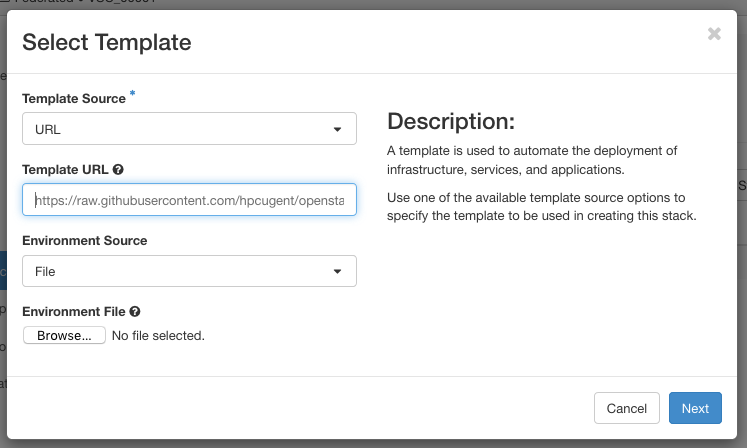
\includegraphics[width=0.7\textwidth]{img/launch_stack_template}
\end{center}
If the template uses parameters, we can specify their values on the
next page of the wizard.  In our example, \strong{nfs\_mount\_point},
\strong{ssh\_user\_key} and \strong{user\_network} are the template
parameters.
\begin{center}
  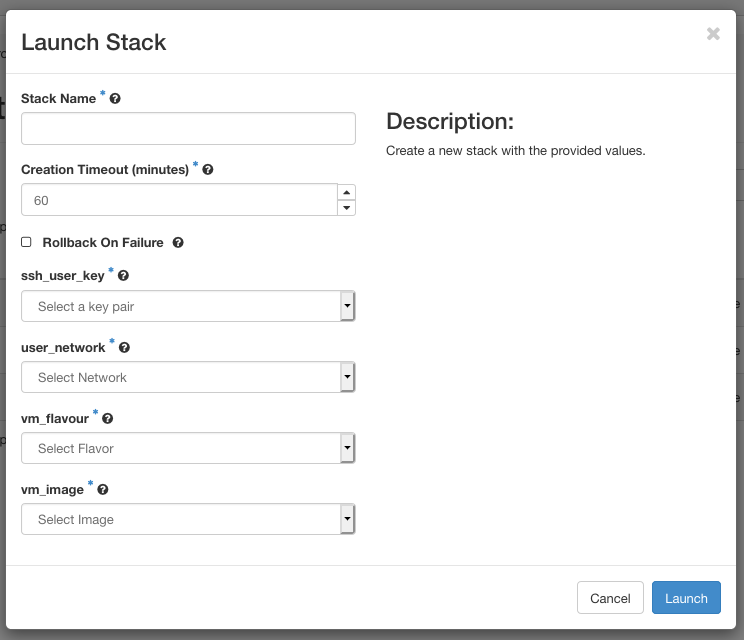
\includegraphics[width=0.7\textwidth]{img/launch_stack_parameters}
\end{center}
Finally, press the Launch button to create the stack.

%%% Local Variables:
%%% mode: latex
%%% TeX-master: "intro-Cloud"
%%% End:
